%!TEX encoding = UTF-8 Unicode
\documentclass{lecturehandouts}

\setbeamertemplate{footline}[frame number]
\title[Föreläsningsanteckningar pgk, 2016]{Programmering, grundkurs \code{pgk}}
\subtitle{Föreläsningsanteckningar \code{pgk} (EDAA45)}
\author{Björn Regnell}
\institute{Datavetenskap, LTH}
\date{Lp1-2, HT 2016}
 
\begin{document}

%\renewcommand{\pause}{}

\newcommand{\Lecture}[2]{%
\section[Vecka #1: #2]{#2}%
\frame{\tableofcontents[currentsubsection,hideothersubsections]}}

\frame{\titlepage}
\frame{\tableofcontents[subsectionstyle=hide]}

\Lecture{1}{Introduktion}
%!TEX encoding = UTF-8 Unicode
%!TEX root = ../lect-week01.tex

%%%%%%%%%%%%%%%%%%%%%%%%%%%%%%%%%%%%%%
\Subsection{Om kursen}

%%%

\ifkompendium\else
\begin{Slide}{Nytt för i år 2016}
\begin{itemize}
\item \Emph{Scala} införs som förstaspråk på Datateknikprogrammet.
\item Den \Emph{största förnyelsen} av den inledande programmeringskursen sedan vi införde \Alert{Java 1997}.
  \begin{itemize}
    \item Nya föreläsningar
    \item Nya övningar
    \item Nya laborationer
    \item Nya skrivningar
  \end{itemize}
\item Allt kursmaterial är \Emph{öppen källkod}.
\item \Emph{Studentermedverkan} i kursutvecklingen.
\end{itemize}
\vspace{1em}\hskip1em\href{https://www.lth.se/nyheter-och-press/nyheter/visa-nyhet/article/scala-blir-foerstaspraak-paa-datateknikprogrammet/}{www.lth.se/nyheter-och-press/nyheter/visa-nyhet/article/\\\hskip1emscala-blir-foerstaspraak-paa-datateknikprogrammet/}
\end{Slide}
\fi

\begin{Slide}{Veckoöversikt}
\noindent\resizebox{0.9\columnwidth}{!}{
\begin{tabular}{l|l|l|l}
\textit{W} & \textit{Modul} & \textit{Övn} & \textit{Lab} \\ \hline \hline
W01 & Introduktion         & expressions & kojo            \\
W02 & Kodstrukturer        & programs    & --              \\
W03 & Funktioner, Objekt   & functions   & simplewindow    \\
W04 & Datastrukturer       & data        & textfiles       \\
W05 & Vektoralgoritmer     & vectors     & cardgame        \\
W06 & Klasser, Likhet      & classes     & shapes          \\
W07 & Arv, Gränssnitt      & traits      & turtlerace-team \\
KS  & KONTROLLSKRIVN.      & --          & --              \\
W08 & Mönster, Undantag    & matching    & chords-team     \\
W09 & Matriser             & matrices    & maze            \\
W10 & Sökning, Sortering   & sorting     & surveydata-team \\
W11 & Scala och Java       & scalajava   & scalajava-team  \\
W12 & Trådar, Web, Android & threads     & life            \\
W13 & Design               & Uppsamling  & Inl.Uppg.       \\
W14 & Tentaträning         & Extenta     & --              \\
T   & TENTAMEN             & --          & --              \\
\end{tabular}

}
\end{Slide}

\ifkompendium
\noindent Kursen består av en \textbf{modul} per läsvecka med två \textbf{föreläsningar}, en \textbf{övning} och en \textbf{laboration} (undantaget W02, W13 \& W14 som saknar labb och/eller övning). 
Föreläsningarna ger en översikt av den teori som ingår i varje modul. Genom att göra övningarna bearbetar du teorin och förebereder dig inför laborationerna. När du klarat övningen och laborationen i en modul är du redo att gå vidare till nästa. Tabellen på nästa uppslag visar begrepp som ingår i varje modul. 

Kursen är uppdelad i två läsperioder. Efter första läsperioden gör du en diagnostisk \textbf{kontrollskrivning} som kontrollerar ditt kunskapsläge. Andra läsperioden avslutas med ett större \textbf{projekt} och en skriftlig \textbf{tentamen}.



\clearpage
\hyphenation{intro-duktion sekvens-algoritmer kod-strukturer data-strukturer}
{\fontsize{11}{13}\selectfont\renewcommand{\arraystretch}{1.75}
\begin{longtable}{@{}p{.05\textwidth} | >{\hspace{0.1em}\raggedright\bfseries\sffamily}p{.15\textwidth}  >{\raggedleft\arraybackslash\hspace{0.0em}\fontsize{10.5}{12}\selectfont}p{0.735\textwidth}}
W01 & Introduktion & sekvens, alternativ, repetition, abstraktion, programmeringsspråk, programmeringsparadigmer, editera-kompilera-exekvera, datorns delar, virtuell maskin, REPL, literal, värde, uttryck, identifierare, variabel, typ, tilldelning, namn, val, var, def, inbyggda typer, Int, Long, Short, Double, Float, Byte, Char, String, println, typen Unit, enhetsvärdet (), stränginterpolatorn s, if, else, true, false, MinValue, MaxValue, aritmetik, slumptal, math.random, logiska uttryck, de Morgans lagar, while-sats, for-sats \\
W02 & Kodstrukturer & iterering, for-uttryck, map, foreach, Range, Array, Vector, algoritm vs implementation, pseudokod, algoritm: SWAP, algoritm: SUM, algoritm: MIN/MAX, algoritm: MININDEX, block, namnsynlighet, namnöverskuggning, lokala variabler, paket, import, filstruktur, jar, dokumentation, programlayout, JDK, main i Java vs Scala, java.lang.System.out.println \\
W03 & Funktioner, objekt & definera funktion, anropa funktion, parameter, returtyp, värdeandrop, namnanrop, default-argument, namngivna argument, applicera funktion på alla element i en samling, procedur, värdeanrop vs namnanrop, uppdelad parameterlista, skapa egen kontrollstruktur, objekt, modul, punktnotation, tillstånd, metod, medlem, funktionsvärde, funktionstyp, äkta funktion, stegad funktion, apply, lazy val, lokala funktioner, anonyma funktioner, lambda, aktiveringspost, anropsstacken, objektheapen, rekursion  cslib.window.SimpleWindow \\
W04 & Datastrukturer & attribut (fält), medlem, metod, tupel, klass, Any, isInstanceOf, toString, case-klass, samling, scala.collection, föränderlighet vs oföränderlighet, List, Vector, Set, Map, typparameter, generisk samling som parameter, översikt samlingsmetoder, översikt strängmetoder, läsa/skriva textfiler, Source.fromFile, java.nio.file \\
W05 & Sekvensalgoritmer & sekvensalgoritm, algoritm: SEQ-COPY, in-place vs copy, algoritm: SEQ-REVERSE, algoritm: SEQ-REGISTER, sekvenser i Java vs Scala, for-sats i Java, java.util.Scanner, scala.collection.mutable.ArrayBuffer, StringBuilder, java.util.Random, slumptalsfrö \\
W06 & Klasser & objektorientering, klass, Point, Square, Complex, new, null, this, inkapsling, accessregler, private, private[this], kompanjonsobjekt, getters och setters, klassparameter, primär konstruktor, objektfabriksmetod, överlagring av metoder, referenslikhet vs strukturlikhet, eq vs == \\
W07 & Arv & arv, polymorfism, trait, extends, asInstanceOf, with, inmixning, supertyp, subtyp, bastyp, override, klasshierarkin i Scala: Any AnyRef Object AnyVal Null Nothing, referenstyper vs värdetyper, klasshierarkin i scala.collection, Shape som bastyp till Point och Rectangle, accessregler vid arv, protected, final, klass vs trait, abstract class, case-object, typer med uppräknade värden \\
KS & \multicolumn{2}{l}{KONTROLLSKRIVN.} \\
W08 & Mönster, undantag & mönstermatchning, match, Option, throw, try, catch, Try, unapply, sealed, flatten, flatMap, partiella funktioner, collect, speciella matchningar: wildcard pattern; variable binding; sequence wildcard; back-ticks, equals, hashcode, exempel: equals för klassen Complex, switch-sats i Java \\
W09 & Matriser, typparametrar & matris, nästlad samling, nästlad for-sats, typparameter, generisk funktion, generisk klass, fri vs bunden typparameter, matriser i Java vs Scala, allokering av nästlade arrayer i Scala och Java \\
W10 & Sökning, sortering & strängjämförelse, compareTo, imlicit ordning, linjärsökning, binärsökning, algoritm: LINEAR-SEARCH, algortim: BINARY-SEARCH, algoritmisk komplexitet, sortering till ny vektor, sortering på plats, insättningssortering, urvalssortering, algoritm: INSERTION-SORT, algoritm: SELECTION-SORT, Ordering[T], Ordered[T], Comparator[T], Comparable[T] \\
W11 & Scala och Java & syntaxskillnader mellan Scala och Java, klasser i Scala vs Java, referensvariabler vs enkla värden i Java, referenstilldelning vs värdetilldelning i Java, alternativ konstruktor i Scala och Java, for-sats i Java, java for-each i Java, java.util.ArrayList, autoboxing i Java, primitiva typer i Java, wrapperklasser i Java, samlingar i Java vs Scala, scala.collection.JavaConverters, namnkonventioner för konstanter \\
W12 & Trådar, webb & tråd, jämlöpande exekvering, icke-blockerande anrop, callback, java.lang.Thread, java.util.concurrent.atomic.AtomicInteger, scala.concurrent.Future, kort om html+css+javascript+scala.js och webbprogrammering \\
W13 & Design, api & utvecklingsprocessen, krav-design-implementation-test, gränssnitt, trait vs interface, programmeringsgränssnitt (api), designexempel \\
W14 & \multicolumn{2}{l}{Tentaträning} \\
T & \multicolumn{2}{l}{TENTAMEN} \\
\end{longtable}
}
\fi

\begin{Slide}{Vad lär du dig?}
\begin{itemize}
\item Grundläggande principer för programmering:\\ Sekvens, Alternativ, Repetition, Abstraktion (SARA)\\$\implies$Inga förkunskaper i programmering krävs!
\item Implementation av algoritmer
\item Tänka i abstraktioner, dela upp problem i delproblem
\item Förståelse för flera olika angreppssätt: 
\begin{itemize}
\item \Emph{imperativ programmering}%: satser, föränderlighet
\item \Emph{objektorientering}%: inkapsling, återanvändning
\item \Emph{funktionsprogrammering}%: uttryck, oföränderlighet
\end{itemize}
\item Programspråken \Emph{Scala} och \Emph{Java}
\item Utvecklingsverktyg (editor, kompilator, utvecklingsmiljö)
\item Implementera, testa, felsöka
\end{itemize}
\end{Slide}


\begin{Slide}{Varför Scala + Java som förstaspråk?}
\begin{itemize}
\item Varför Scala?
\begin{itemize}
\item Enkel och enhetlig syntax => lätt att skriva
\item Enkel och enhetlig semantik => lätt att fatta 
\item Kombinerar flera angreppsätt => lätt att visa olika lösningar
\item Statisk typning + typhärledning =>  färre buggar + koncis kod
\item Scala Read-Evaluate-Print-Loop => lätt att experimentera
\end{itemize}


\item Varför Java?
\begin{itemize}
\item Det mest spridda språket
\item Massor av fritt tillgängliga kodbibliotek
\item Kompabilitet: fungerar på många platformar
\item Effektivitet: avancerad \& mogen teknik ger snabba program
\end{itemize}
\item Java och Scala fungerar utmärkt tillsammans
\item Illustrera likheter och skillnader mellan olika språk \\ => Djupare lärande
\end{itemize}
\end{Slide}


\begin{Slide}{Hur lär du dig?}
\begin{itemize}
\item Genom praktiskt \Alert{eget arbete}: \Emph{Lära genom att göra!}
\begin{itemize}
\item Övningar: applicera koncept på olika sätt
\item Laborationer: kombinera flera koncept till en helhet
\end{itemize}
\item Genom studier av kursens teori: \Emph{Skapa förståelse!}
\item Genom samarbete med dina kurskamrater: \Emph{Gå djupare!}
\end{itemize}
\end{Slide}


\begin{Slide}{Kurslitteratur}
\begin{minipage}{0.45\textwidth}\SlideFontSmall
\hskip1.33em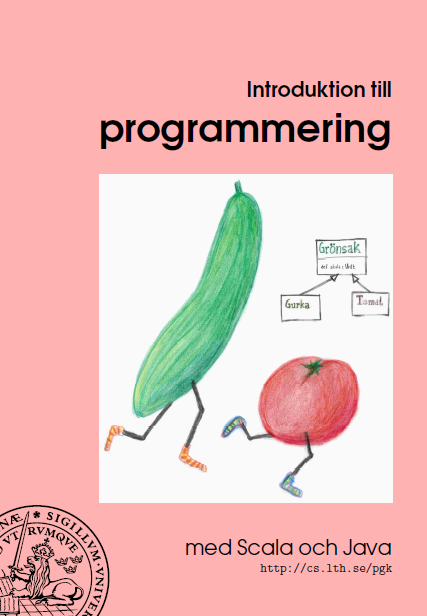
\includegraphics[width=0.65\textwidth]{../img/compendium-front-page.png}
\begin{itemize}
\item \Emph{Kompendium} med övningar \& laborationer, trycks \& säljs av inst. på beställning
\item Föreläsningsbilder
\item Nätresurser enl. länkar

\end{itemize}
\end{minipage}
\hskip1em\begin{minipage}{0.5\textwidth}\SlideFontSize{8}{10}
Bra, men ej nödvändig, \Emph{bredvidläsning}:\\ 
-- för \Emph{nybörjare}:
\vskip0.2mm

\includegraphics[width=0.33\textwidth]{../img/lewisbook.jpg}\hskip4mm

\includegraphics[width=0.33\textwidth]{../img/ankbok.jpg}

\noindent -- för de som \Emph{redan kodat} en del:
\vskip0.7mm
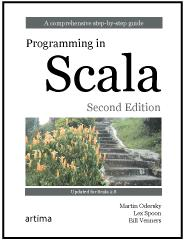
\includegraphics[width=0.45\textwidth]{../img/pinsbook.jpg}\hskip4mm

\includegraphics[width=0.47\textwidth]{../img/koffmanbook.jpg}
\end{minipage}
\end{Slide}

\ifkompendium
\noindent Kompendiet är den huvudsakliga kurslitteraturen och definierar kursinnehållet. Föreläsningar, övningar och laborationer i kompendiet är kursens primära kunskapskällor, tillsammans med de öppna resurser på nätet som kompendiet hänvisar till. Kompendiet är öppen källkod och du välkomnas varmt att bidra!

Om du gärna vill ha en eller flera mer traditionella läroböcker som bredvidläsning rekommenderas följande:
\begin{itemize}[noitemsep, leftmargin=*]
\item För de som aldrig kodat, och vill läsa om kodning från grunden:
\begin{itemize}[nolistsep]
\item ''Introduction to Programming and Problem-Solving Using Scala, Second Edition'', Mark C. Lewis, Lisa Lacher.  {\href{https://www.crcpress.com/Introduction-to-Programming-and-Problem-Solving-Using-Scala-Second-Edition/Lewis-Lacher/p/book/9781498730952}{www.crcpress.com/Introduction-to-Programming-and-Problem-Solving-Using-Scala-Second-Edition/Lewis-Lacher/p/book/9781498730952}}
\item ''Objektorienterad programmering och Java'', Per Holm, Tredje upplagan (2007). \href{https://www.studentlitteratur.se/#6735}{www.studentlitteratur.se/\#6735}
\end{itemize}
\item För de som redan kodat en hel del i ett objektorienterat språk:
\begin{itemize}[nolistsep, noitemsep]
\item ''Programming in Scala, Third Edition -- A comprehensive step-by-step guide'', Martin Odersky, Lex Spoon, and Bill Venners. \\ \href{http://www.artima.com/shop/programming_in_scala_3ed}{www.artima.com/shop/programming\_in\_scala\_3ed} 
\item ''Data Structures: Abstraction and Design Using Java, 3rd Edition'', Elliot B. Koffman, Paul A. T. Wolfgang. \\
\href{http://eu.wiley.com/WileyCDA/WileyTitle/productCd-1119186528.html}{http://eu.wiley.com/WileyCDA/WileyTitle/productCd-1119186528.html}
\end{itemize}
\end{itemize}
Dessa läroböcker följer inte direkt kursens upplägg vad gäller omfång och progression och du får själv göra den nyttiga hemläxan att koppla  deras innehåll till det vi går igenom i kursens olika moduler.

\else


\begin{Slide}{Beställning av kompendium och snabbreferens}\SlideFontSmall
\begin{itemize}

\item \Emph{Kompendiet} finns i pdf för fri nedladdning enl. CC-BY-SA, men det \Alert{rekommenderas starkt} att du köper den tryckta bokversionen.

\item Det är mycket lättare att ha övningar och labbar \Alert{på papper} \Emph{bredvid skärmen}, när du ska tänka, koda och plugga!

\item \Emph{Snabbreferensen} finns också i pdf men du behöver ha en tryckt version eftersom det är \Alert{enda tillåtna hjälpmedlet} på skriftliga kontrollskrivningen och tentamen.

\item Kompendiet och snabbreferens trycks här i E-huset och säljs av institutionen till \Emph{självkostnadspris}. 

\item Pris för kompendium \Alert{beror på hur många som beställer}.

\item Snabbreferens kostar 10 kr.

\item Kryssa i \Alert{BOK} på listan som snart skickas runt -- tryckning enligt denna beställning.

\item Du betalar \Alert{kontant} med \Emph{jämna pengar} på cs expedition, våning 2.

\end{itemize}
\end{Slide}

\fi


\begin{Slide}{Föreläsningsanteckningar}
\begin{itemize}
\item Föreläsningbilder utvecklas under kursens gång.
\item Alla bilder läggs ut här: \\
\href{https://github.com/lunduniversity/introprog/tree/master/slides}{github.com/lunduniversity/introprog/tree/master/slides} \\
och uppdateras kontinuerligt allt eftersom de utvecklas.
\item Förslag på innehåll välkomna!
\end{itemize}
\end{Slide}


\ifkompendium\else
\begin{Slide}{Personal}\SlideFontSmall
\begin{description}
\item [\bfseries Kursansvarig:] ~\\Björn Regnell, bjorn.regnell@cs.lth.se
\item [\bfseries Kurssekreterare:]  ~\\Lena Ohlsson \\Exp.tid 09.30 -- 11.30 samt 12.45 -- 13.30
\item [\bfseries Handledare:] ~\\
\Emph{Doktorander}: \\ 
MSc. Gustav Cedersjö, Tekn. Lic. Maj Stenmark \\
\Emph{Teknologer}: \\
Anders Buhl, 
Anna Palmqvist Sjövall, 
Anton Andersson,
Cecilia Lindskog, 
Emil Wihlander, 
Erik Bjäreholt, 
Erik Grampp, 
Filip Stjernström, 
Fredrik Danebjer, 
Henrik Olsson, 
Jakob Hök, 
Jonas Danebjer, 
Måns Magnusson, 
Oscar Sigurdsson, 
Oskar Berg, 
Oskar Widmark, 
Sebastian Hegardt, 
Stefan Jonsson, 
Tom Postema, 
Valthor Halldorsson
\end{description}
\end{Slide}
\fi


\begin{Slide}{Kursmoment --- varför?}\SlideOnly{\footnotesize}
\begin{itemize}

\item \Emph{Föreläsningar}: skapa översikt, ge struktur, förklara teori, svara på frågor, motivera varför.

\item \Emph{Övningar}: bearbeta teorins steg för steg, \Emph{grundövningar} för alla, \Emph{extraövningar} om du vill/behöver öva mer, \Emph{fördjupningsövningar} om du vill gå djupare; \Alert{förberedelse inför laborationerna}.
 
\item \Emph{Laborationer}: \Alert{obligatoriska}, sätta samman teorins delar i ett större program; lösningar redovisas för handledare; gk på alla för att få tenta.

\item \Emph{Resurstider}: få hjälp med övningar och laborationsförberedelser av handledare, fråga vad du vill.

\item \Emph{Samarbetsgrupper}: grupplärande genom samarbete, hjälpa varandra.

\item \Emph{Kontrollskrivning}: \Alert{obligatorisk}, diagnostisk, kamraträttad; kan ge samarbetsbonuspoäng till tentan.

\item \Emph{Individuell projektuppgift}: \Alert{obligatorisk}, du visar att du kan skapa ett större program självständigt; redovisas för handledare.

\item \Emph{Tentamen}: \Alert{obligatorisk}, skriftlig, enda hjälpmedel: snabbreferensen.\\   \url{http://cs.lth.se/pgk/quickref}
\end{itemize}
\end{Slide}

\ifkompendium\else
\begin{Slide}{Detta är bara början... }
Exempel på efterföljande kurser som bygger vidare på denna:
\begin{itemize}
\item \Emph{Årskurs 1}
\begin{itemize}
\item Programmeringsteknik -- fördjupningskurs
\item Utvärdering av programvarusystem
\item Diskreta strukturer
\end{itemize}
\item \Alert{Årskurs 2}
\begin{itemize}
\item Objektorienterad modellering och design
\item Programvaruutveckling i grupp
\item Algoritmer, datastrukturer och komplexitet
\item Funktionsprogrammering
\end{itemize}
\end{itemize}
\end{Slide}


\begin{Slide}{Registrering}
\begin{itemize}
\item Fyll i listan \Emph{REGISTRERING EDAA45} som skickas runt.

\item Kryssa i kolumnen \Alert{ÅBEROPAR PLATS} om vill gå kursen\footnote{\scriptsize D1:a som redan gått motsvarande högskolekurs? Uppsök studievägledningen}\footnote{\scriptsize D2:a eller äldre som redan påbörjad EDA016/EDA011/EDA017 el likn.? Övergångsregler: Alla labbar gk: tenta EDA011/017; annars kom och prata på rasten}

\item Kryssa i kolumnen \Emph{BESTÄLLER BOK} 

\item Kryssa i kolumnen \Emph{KAN VARA KURSOMBUD} om du kan tänka dig att vara kursombud under kursens gång:
\begin{itemize}
\item Alla LTH-kurser ska utvärderas under kursens gång och efter kursens slut.
\item Till det behövs kursombud -- ungefär \Alert{2 D-are} och \Alert{2 W-are}.
\item Ni kommer att bli kontaktade av studierådet. 
\end{itemize}
\end{itemize}
\end{Slide}

%%%
\begin{Slide}{Förkunskaper}
\begin{itemize}
\item Förkunskaper $\neq$ Förmåga
\item Varken kompetens eller personliga egenskaper är statiska 
\item ''Programmeringskompetens'' är inte \textit{en} enda enkel förmåga utan en komplex sammansättning av flera olika förmågor som \Emph{utvecklas} genom hela livet
\item Ett innovativt utvecklar\Alert{team} behöver många olika kompetenser för att vara framgångsrikt
\end{itemize}
\end{Slide}

%%%
\begin{Slide}{Förkunskapsenkät}
\begin{itemize}
\item Om du inte redan gjort det fyll i förkunskapsenkäten \Alert{snarast}:
\url{http://cs.lth.se/pgk/survey} 
\item Dina svar behandlas internt och all redovisad statistik anonymiseras.
\item Enkäten ligger till grund för randomiserad gruppindelning i samarbetsgrupper, så att det blir en spridning av förkunskaper inom gruppen.
\item Gruppindelnig publiceras här: \\ \url{http://cs.lth.se/pgk/grupper/}
\end{itemize}
\end{Slide}

\begin{Slide}{Samarbetgrupper}\footnotesize
\begin{itemize}
\item Ni delas in i \Emph{samarbetsgrupper} om ca 5 personer baserat på förkunskapsenkäten, så att olika förkunskapsnivåer sammanförs
\item Några av laborationerna är mer omfattande \Emph{grupplabbar} och kommer att göras i samarbetsgrupperna \\ \vspace{1em}
\item Kontrollskrivningen i halvtid kan ge \Emph{samarbetsbonus} (max 5p) som adderas till ordinarie tentans poäng (max 100p) med medelvärdet av gruppmedlemmarnas individuella kontrollskrivningspoäng 
\scriptsize \parbox{7cm}{Bonus $b$ för varje person i en grupp med $n$ medlemmar med $p_i$ poäng vardera på kontrollskrivningen:} 
 \hspace{5mm} $\displaystyle b = \sum\limits_{i=1}^n \frac{p_i}{n}$
\end{itemize}
\end{Slide}

\fi

%%%
\begin{Slide}{Varför studera i samarbetsgrupper?}

Huvudsyfte: \Emph{Bra lärande!}

\begin{itemize}
\item Pedagogisk forskning stödjer tesen att lärandet blir mer djupinriktat om det sker i utbyte med andra
\item Ett studiesammanhang med \Alert{höga ambitioner} och \Alert{respektfull gemenskap} gör att vi \Emph{når mycket längre}
\item Varför ska du som redan kan mycket aktivt dela med dig av dina kunskaper?
\begin{itemize}
\item Förstå bättre själv genom att förklara för andra
\item Träna din pedagogiska förmåga
\item Förbered dig för ditt kommande yrkesliv som mjukvaruutvecklare 
\end{itemize}
\end{itemize}
\end{Slide}

%%%

\ifkompendium\else
\begin{Slide}{Samarbetskontrakt}
Gör ett skriftligt \href{https://github.com/lunduniversity/introprog/tree/master/admin}{\Emph{samarbetskontrakt}} med dessa och ev. andra punkter som ni också tycker bör ingå:
\begin{enumerate}
\item Återkommande mötestider per vecka
\item Kom i tid till gruppmöten
\item Var väl förberedd genom självstudier inför gruppmöten
\item Hjälp varandra att förstå, men ta inte över och lös allt
\item Ha ett respektfullt bemötande även om ni har olika åsikter
\item Inkludera alla i gemenskapen
\end{enumerate}

Diskutera hur ni ska uppfylla dessa innan alla skriver på. \\ Ta med samarbetskontraktet och visa för handledare på labb 1.

\vskip1em

\Alert{Om arbetet i samarbetsgruppen inte fungerar ska ni mejla kursansvarig och boka mötestid!}
\end{Slide}

\begin{Slide}{Bestraffa inte frågor!}
\begin{itemize}
\item Det finns bättre och sämre frågor vad gäller hur mycket man kan lära sig av svaret, men \Emph{all undran är en chans} att i dialog utbyta erfarenheter och lärande
\item Den som frågar \Emph{vill veta} och berättar genom frågan något om nuvarande kunskapsläge
\item Den som svarar får chansen att \Emph{reflektera} över vad som kan vara svårt och olika vägar till djupare förståelse
\item I en hälsosam lärandemiljö är det \Emph{helt tryggt} att visa att man ännu inte förstår, att man gjort ''fel'', att man har mer att lära, etc. 
\item Det är viktigt att våga försöka även om det blir ''fel'':\\ \Emph{det är ju då man lär sig!}
\end{itemize}
\end{Slide}

%%%
\begin{Slide}{Plagiatregler}
Läs dessa regler noga och diskutera i samarbetsgrupperna:
\begin{itemize}
\footnotesize
\item \url{http://cs.lth.se/utbildning/samarbete-eller-fusk/}
\item \href{http://cs.lth.se/utbildning/foereskrifter-angaaende-obligatoriska-moment/}{Föreskrifter angående obligatoriska moment}
\end{itemize}
Ni ska lära er genom \Emph{eget arbete} och genom  \Emph{bra samarbete}. Samarbete gör att man lär sig bättre, men man lär sig inte av att bara kopiera andras lösningar. \Alert{Plagiering är förbjuden} och kan medföra \Alert{disciplinärende och avstängning}.
\end{Slide}

\fi %%%%%%%%%%%%%%%%%%%%%%%%%%%%%%%%

%%%
\begin{Slide}{En typisk kursvecka}
\begin{enumerate}
\item Gå på \Emph{föreläsningar} på \Alert{måndag--tisdag}
\item \Alert{Jobba} \Emph{individuellt} med teori, övningar, labbförberedelser på  \Alert{måndag--torsdag}
\item Kom till \Emph{resurstiderna} och få hjälp och tips av handledare och kurskamrater på \Alert{onsdag--torsdag}
\item Genomför den obligatoriska \Emph{laborationen} på \Alert{fredag}
\item \Alert{Träffas} i \Emph{samarbetsgruppen} och hjälp varandra att förstå mer och fördjupa lärandet, förslagsvis på återkommande tider varje vecka då alla i gruppen kan
\end{enumerate}
Se detaljerna och undantagen i schemat: \href{http://cs.lth.se/pgk/schema}{cs.lth.se/pgk/schema}
\end{Slide}

\ifkompendium\else  %%%%%%%%%%%%%%%%%%%%%%%%%
%%%
\begin{Slide}{Laborationer}\footnotesize
\begin{itemize}
\item \Alert{Programmering lär man sig bäst genom att programmera...}

\item Labbarna är \Emph{individuella} (utom 3) och \Emph{obligatoriska}

\item Gör \Emph{övningarna} och \Emph{labbförberedelserna} noga \Alert{innan} själva labben -- detta är ofta helt nödvändigt för att du ska hinna klart. Dina labbförberedelserna kontrolleras av handledare under labben.

\item Är du \Emph{sjuk?} Anmäl det \Alert{före} labben till \url{bjorn.regnell@cs.lth.se}, \\ få hjälp på resurstid och redovisa på resurstid (eller labbtid, när handledaren har tid över)

\item Hinner du inte med hela labben? Se till att handledaren \Emph{noterar din närvaro}, och fortsätt på resurstid och ev. uppsamlingstider.

\item Läs noga kapitel noll ''\Alert{Anvisningar}'' i kompendiet!

\item Laborationstiderna är gruppindelade enligt \href{http://cs.lth.se/pgk/schema/}{schemat}. Du ska gå till den tid och den sal som motsvarar din grupp som visas i \href{http://cs.lth.se/pgk/schema/timeedit}{TimeEdit}. \Emph{Gruppindelning} meddelas på hemsidan senast onsdag morgon.
\end{itemize}
\end{Slide}

%%%
\begin{Slide}{Resurstider}\SlideFontSmall
\begin{itemize}
\item På resurstiderna får du \Emph{hjälp}  med \Alert{övningar} och labb\Alert{förberedelser}.

\item Kom till minst en resurstid per vecka, se \href{http://cs.lth.se/pgk/schema/timedit}{TimeEdit}.

\item Handledare gör ibland \Emph{genomgångar} för alla under resurstiderna. Tipsa om handledare om vad du finner svårt!
\item Du får i mån av plats gå på flera resurstider per vecka. Om det blir fullt i ett rum prioriteras schemagrupper för att minimera krockar: 
\end{itemize}
\begin{table}[]
\centering\scriptsize
\begin{tabular}{lllll}
\Emph{Tid Lp1} & \Emph{Sal} & \Alert{Grupper med prio} \\
\hline
Ons 10-12 v1-7 & Falk &   09 \\
Ons 10-12 v1-7 & Val  &   10 \\
Ons 13-15 v1-7 & Falk &   03 \\
Ons 13-15 v1-7 & Val  &   04 \\
Ons 15-17 v1-7 & Falk &   11 \\
Ons 15-17 v1-7 & Val  &   12 \\ \hline
Tor 10-12 v1-7 & Falk &   01 \\
Tor 10-12 v1-7 & Val  &   02 \\
Tor 13-15 v1-7 & Falk &   05 \\
Tor 13-15 v1-7 & Val  &   06 \\
Tor 15-17 v1-7 & Falk &   07 \\
Tor 15-17 v1-7 & Val  &   08 \\
\end{tabular}
\end{table}
\end{Slide}

\fi
%!TEX encoding = UTF-8 Unicode
%!TEX root = ../lect-week01.tex

%%%%%%%%%%%%%%%%%%%%%%%%%%%%%%%%%%%%%%

\Subsection{Att lära denna läsvecka \texttt{w01}}

\ifkompendium\else  %%%%%%%%%%%%%%%%%%%%%%%%%%%%%%%%%%%%%%%%%%%%%%%%%
\begin{Slide}{Att lära denna läsvecka \texttt{w01}}
%!TEX encoding = UTF-8 Unicode

Modul \Emph{Introduktion}: Övn \Alert{\texttt{expressions}} $\rightarrow$ Labb \Alert{\texttt{kojo}}
\begin{multicols}{3}\SlideFontTiny
$\square$ sekvens \\
$\square$ alternativ \\
$\square$ repetition \\
$\square$ abstraktion \\
$\square$ programmeringsspråk \\
$\square$ programmeringsparadigmer \\
$\square$ editera-kompilera-exekvera \\
$\square$ datorns delar \\
$\square$ virtuell maskin \\
$\square$ REPL \\
$\square$ literal \\
$\square$ värde \\
$\square$ uttryck \\
$\square$ identifierare \\
$\square$ variabel \\
$\square$ typ \\
$\square$ tilldelning \\
$\square$ namn \\
$\square$ val \\
$\square$ var \\
$\square$ def \\
$\square$ inbyggda grundtyper \\
$\square$ Int \\
$\square$ Long \\
$\square$ Short \\
$\square$ Double \\
$\square$ Float \\
$\square$ Byte \\
$\square$ Char \\
$\square$ String \\
$\square$ println \\
$\square$ typen Unit \\
$\square$ enhetsvärdet () \\
$\square$ stränginterpolatorn s \\
$\square$ if \\
$\square$ else \\
$\square$ true \\
$\square$ false \\
$\square$ MinValue \\
$\square$ MaxValue \\
$\square$ aritmetik \\
$\square$ slumptal \\
$\square$ math.random \\
$\square$ logiska uttryck \\
$\square$ de Morgans lagar \\
$\square$ while-sats \\
$\square$ for-sats \\     
\end{multicols}

\end{Slide}
\fi

\Subsection{Om programmering}

\ifkompendium\else
\SlideImg{Programming unplugged: Två frivilliga?}{../img/unplugged}
\SlideImg{Editera och exekvera ett program}{../img/kojo}
\fi

%%%

\ifkompendium\else
\SlideImg{Vad är en dator?}{../img/eniac}


\begin{Slide}{Hur fungerar en dator?}
\begin{tikzpicture}[node distance=2.0cm]
\node (input)  [startstop]               {Indata-enhet};
\node (cpu)    [process, below of=input] {CPU};
\node (output) [startstop,below of=cpu]  {Utdata-enhet};

\node (mem) [right of=cpu, xshift=4cm, draw = black, thick] {
\begin{minipage}{0.5\textwidth}\centering
\textbf{Minne} med minnesceller
\vspace{1em}

\begin{tabular}{|l | l|}
address & innehåll \\ \hline
0   & 42 \\ \hline
1   & 13 \\ \hline
2   & 18 \\ \hline
3   & 21 \\ \hline
4   & 55 \\ \hline
5   & 64 \\ \hline
6   & 48 \\ \hline 
... & ...
\end{tabular}
\end{minipage}
};

\draw [arrow] (input) -- (cpu);
\draw [arrow] (cpu) -- (output);
\draw [arrow] (cpu) -- (mem);
\draw [arrow] (mem) -- (cpu);

\node(memtext) [below of=mem, text width=7.0cm, scale=0.8, yshift=-1.5cm, xshift=0.5cm ] 
{Minnet innehåller endast \Alert{heltal} som \newline representerar \Emph{data} \Alert{och} \Emph{instruktioner}.};

%\node(memtext) [right of=input, text width=2cm, scale=0.8,xshift=1.0cm]{För\\människor};
%\node(output) [right of=output, text width=2cm, scale=0.8,xshift=1.0cm]{För\\maskiner};
\end{tikzpicture}
\end{Slide}

\fi

\begin{Slide}{Vad är programmering?}
\begin{itemize}
\item Programmering innebär att ge instruktioner till en maskin.
\item Ett \Emph{programmeringsspråk} används av människor för att skriva \Emph{källkod} som kan översättas av en \Emph{kompilator} till \Emph{maskinspråk} som i sin tur \Emph{exekveras} av en dator.
\end{itemize}


\begin{minipage}{.8\textwidth}
\begin{itemize}
\item Ada Lovelace skrev det första programmet redan på 1800-talet ämnat för en kugghjulsdator. 
\end{itemize}
\end{minipage}%
\begin{minipage}{.2\textwidth}
\centering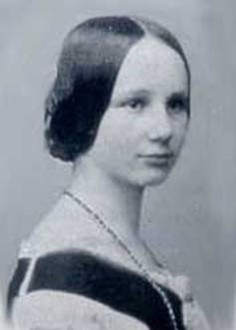
\includegraphics[width=0.6\columnwidth]{../img/ada}
\end{minipage}%
\begin{itemize}
\item \href{https://sv.wikipedia.org/wiki/Programmering}{sv.wikipedia.org/wiki/Programmering}
\item \href{https://en.wikipedia.org/wiki/Computer\_programming}{en.wikipedia.org/wiki/Computer\_programming}
\item Ha picknick i \href{http://kartor.lund.se/wiki/lundanamn/index.php/Ada_Lovelace-parken}{Ada Lovelace-parken} på Brunnshög!
\end{itemize}
\end{Slide}


\begin{Slide}{Vad är en kompilator?}
\begin{multicols}{2}
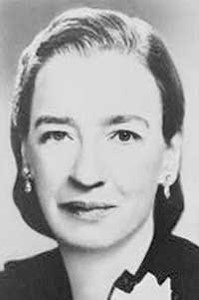
\includegraphics[width=0.8\columnwidth]{../img/grace}

\columnbreak %---------

Grace Hopper uppfann första kompilatorn 1952.\\
\href{https://en.wikipedia.org/wiki/Grace\_Hopper}{\SlideFontTiny en.wikipedia.org/wiki/Grace\_Hopper}
\vskip1em
%https://www.sharelatex.com/blog/2013/08/29/tikz-series-pt3.html
\begin{tikzpicture}[node distance=1.8cm]
\node (input) [startstop] {Källkod};
\node(inptext) [right of=input, text width=2cm, scale=0.8,xshift=1.0cm]{För\\människor};
\node (compile) [process, below of=input] {Kompilator};
\node (output) [startstop, below of=compile] {Maskinkod};
\node(outtext) [right of=output, text width=2cm, scale=0.8,xshift=1.0cm]{För\\maskiner};
\draw [arrow] (input) -- (compile);
\draw [arrow] (compile) -- (output);
\end{tikzpicture}
\end{multicols}
\end{Slide}


\ifkompendium\else

\begin{Slide}{Virtuell maskin (VM) == abstrakt hårdvara}
\begin{multicols}{2}

En VM är en ''dator'' implementerad i mjukvara som kan tolka en generell ''maskinkod'' som \Emph{översätts under körning} till den verkliga maskinens kod. \\
\vspace{1em}
Med en VM blir källkoden \Emph{plattformsoberoende} och fungerar på många olika maskiner. \\
\vspace{1em}
Exempel: \\ \Emph{Java Virtual Machine}
\columnbreak %---------

%https://www.sharelatex.com/blog/2013/08/29/tikz-series-pt3.html
\begin{tikzpicture}[node distance=1.4cm]
\node (input) [startstop] {Källkod};
\node (compile) [process, below of=input] {Kompilator};
\node (output) [startstop, below of=compile] {Generell ''maskinkod''};
\node (interp) [process, below of=output] {VM interpreterar};
\node (output2) [startstop, below of=interp] {Specifik maskinkod};
\draw [arrow] (input) -- (compile);
\draw [arrow] (compile) -- (output);
\draw [arrow] (output) -- (interp);
\draw [arrow] (interp) -- (output2);
\end{tikzpicture}
\end{multicols}
\end{Slide}
\fi

\begin{Slide}{Vad består ett program av?}
\begin{itemize}
\item Text som följer entydiga språkregler (gramatik): 
\begin{itemize}
\item \Emph{Syntax}: textens konkreta utseende 
\item \Emph{Semantik}: textens betydelse (vad maskinen gör/beräknar)
\end{itemize}
\item \Emph{Nyckelord}: ord med speciell betydelse, t.ex. \code{if}, \code{else}
\item \Emph{Deklarationer}: definitioner av nya ord: \code{def gurka = 42}
\item \Emph{Satser} är instruktioner som \emph{gör} något: \code{print("hej")} 
\item \Emph{Uttryck} är instruktioner som beräknar ett \emph{resultat}: \code{1 + 1}
\item \Emph{Data} är information som behandlas: t.ex. heltalet \code{42}
\item Instruktioner ordnas i kodstrukturer: (SARA)
\begin{itemize}
\item \Emph{Sekvens}: ordningen spelar roll för vad som händer
\item \Emph{Alternativ}: olika saker händer beroende på uttrycks värde
\item \Emph{Repetition}: satser upprepas många gånger
\item \Emph{Abstraktion}: nya byggblock skapas för att återanvändas
\end{itemize}
\end{itemize}
\end{Slide}

\begin{Slide}{Exempel på programmeringsspråk}
Det finns massor med olika språk och det kommer ständigt nya. 
\vspace{1em}
\begin{multicols}{2}
Exempel:
\begin{itemize}
\item Java
\item C
\item C++
\item C\#
\item Python
\item JavaScript
\item Scala
\end{itemize}

\columnbreak %---------

Topplistor:
\begin{itemize}
\item \href{http://www.tiobe.com/index.php/content/paperinfo/tpci/index.html}{TIOBE Index}
\item \href{http://pypl.github.io/PYPL.html}{PYPL Index}
\end{itemize}
\vspace{1em}

\includegraphics[width=0.8\columnwidth]{../img/pypl}
\end{multicols}

\end{Slide}


\begin{Slide}{Hello world}

\begin{REPLnonum}
scala> println("Hello World!")
Hello World!
\end{REPLnonum}

\begin{Code}
// this is Scala 

object Hello {
  def main(args: Array[String]): Unit = {
    println("Hejsan scala-appen!")
  }
}
\end{Code}


\begin{Code}[language=Java]
// this is Java 

public class Hi {
    public static void main(String[] args) {
        System.out.println("Hejsan Java-appen!");
    }
}
\end{Code}

\end{Slide}

\begin{Slide}{Utvecklingscykeln}
editera; kompilera; hitta fel och förbättringar; editera; kompilera; hitta fel och förbättringar; editera; kompilera; hitta fel och förbättringar; editera; kompilera; hitta fel och förbättringar; editera; kompilera; hitta fel och förbättringar; editera; kompilera; hitta fel och förbättringar; ...

\begin{Code}
upprepa(1000){
  editera
  kompilera
  testa
}
\end{Code}
\end{Slide}

\begin{Slide}{Utvecklingsverktyg}
\begin{itemize}
\item Din verktygskunskap är mycket viktig för din produktivitet. 
\item Lär dig kortkommandon för vanliga handgrep. 
\item Verktyg vi använder i kursen:
\begin{itemize}
\item Scala \Emph{REPL}: från övn 1
\item \Emph{Texteditor} för kod, t.ex \code{gedit} eller \code{atom}: från övn 2
\item Kompilera med \Emph{\code{scalac}} och \Emph{\code{javac}}: från övn 2
\item Integrerad utvecklingsmiljö (IDE)
\begin{itemize}
\item \Emph{Kojo}: från lab 1
\item \Emph{Eclipse+ScalaIDE} eller \Emph{IntelliJ IDEA} med Scala-plugin: från lab 3 i vecka 4
\end{itemize}
\item \Emph{jar} för att packa ihop och distribuera klassfiler
\item \Emph{javadoc} och \Emph{scaladoc} för dokumentation av kodbibliotek
\end{itemize}
\item Andra verktyg som är bra att lära sig:
\begin{itemize}
\item git för versionshantering
\item GitHub för kodlagring -- men \Alert{inte} av lösningar till labbar!
\end{itemize}
\end{itemize}
\end{Slide}


\ifkompendium\else  %%%%%%%%%%%%%%%%%%%%%%%%%%%%%%%%%%%%%%%%%%%%%%%%%

\begin{Slide}{Att skapa koden som styr världen}
\begin{multicols}{2}\footnotesize
I stort sett alla delar av samhället är beroende av programkod:
\begin{itemize}\scriptsize
\item kommunikation
\item transport
\item byggsektorn
\item statsförvaltning
\item finanssektorn
\item media \& underhållning
\item sjukvård
\item övervakning
\item integritet
\item upphovsrätt
\item miljö \& energi
\item sociala relationer
\item utbildning 
\item ...
\end{itemize}
\columnbreak %---------
Hur blir ditt framtida yrkesliv som systemutvecklare?
\begin{itemize}
\item  Det är sedan lång tid en skriande brist på utvecklare och bristen blir bara värre och värre... \\
  \href{http://computersweden.idg.se/2.2683/1.663879/oppen-kallkod-brist-kompetens}{CS 2016-08-23}
\item Störst brist är det på kvinnliga utvecklare: \\
\href{http://www.dn.se/ekonomi/it-branschen-hotas-av-brist-pa-kvinnor/}{DN 2015-04-02}
\item Global kompetensmarknad \\ 
  \href{http://computersweden.idg.se/2.2683/1.630901/det-finns-programmerare-och-sa-finns-det-programmerare}{CS 2015-06-14} \\
  \href{http://computersweden.idg.se/2.2683/1.662186/25-miljoner-utvecklare?queryText=miljoner\%20utvecklare}{CS 2016-07-14 }
\end{itemize}
\end{multicols}
\end{Slide}

\begin{Slide}{Utveckling av mjukvara i praktiken}
\begin{itemize}
\item \Emph{Inte bara kodning:} kravbeslut, releaseplanering, design, test, versionshantering, kontinuerlig integration, driftsättning, återkoppling från dagens användare, ekonomi \& investering, gissa om morgondagens användare, ... 
\item \Emph{Teamwork:} Inte ensamma hjältar utan autonoma team i decentraliserade organisationer med innovationsuppdrag
\item \Emph{Snabbhet:} Att koda innebär att hela tiden uppfinna nya ''byggstenar'' som ökar organisationens förmåga att snabbt skapa värde med hjälp av mjukvara. Öppen källkod. Skapa kraftfulla API:er.
\item \Emph{Livslångt lärande:} Lär nytt och dela med dig hela tiden. Exempel på pedagogisk utmaning: hjälp andra förstå och använda ditt API $\implies$ \textit{Samarbetskultur}
\end{itemize}
\end{Slide}


\fi %%%%%%%%%%%%%%%%%%%%%%%%%%%%%%%%%%%%%%%%%%%%%%%%%%%%


\Subsection{De enklaste beståndsdelarna: litteraler, uttryck, variabler}


\begin{Slide}{Literaler}
\begin{itemize}
\item Literaler representerar ett fixt \Emph{värde} i koden och används för att skapa \Alert{data} som programmet ska bearbeta.
\item Exempel: \\
\begin{tabular}{l l}
\code|42| & heltalslitteral\\
\code|42.0| & decimaltalslitteral\\
\code|'!'| & teckenlitteral, omgärdas med 'enkelfnuttar' \\
\code|"hej"| & stränglitteral, omgärdas med ''dubbelfnuttar'' \\
\code|true| & litteral för sanningsvärdet ''sant''\\
\end{tabular} 
\item Literaler har en \Emph{typ} som avgör vad man kan göra med dem.
\end{itemize}
\end{Slide}

\begin{Slide}{Exempel på inbyggda datatyper i Scala}
\begin{itemize}
\item Alla värden, uttryck och variabler har en \href{https://sv.wikipedia.org/wiki/Datatyp}{\Emph{datatyp}}, t.ex.: 
\begin{itemize}\footnotesize
\item \code{Int} för heltal 
\item \code{Long} för \textit{extra} stora heltal (tar mer minne)
\item \code{Double} för decimaltal, så kallade flyttal med flytande decimalpunkt
\item \code{String} för strängar
\end{itemize}
\item Kompilatorn håller reda på att uttryck kombineras på ett \Emph{typsäkert} sätt. Annars blir det kompileringsfel.
\item Scala och Java är s.k. \href{https://sv.wikipedia.org/wiki/Typsystem}{\Emph{statiskt typade}} språk, vilket innebär att all typinformation måste finnas redan vid kompileringsdags \Eng{compile time}\footnote{Andra språk, t.ex. Python och Javascript är dynamiskt typade och där skjuts typkontrollen upp till körningsdags \Eng{run time} \\ Vilka är för- och nackdelarna med statisk vs. dynamisk typning?}. 
\end{itemize}
\end{Slide}


\begin{Slide}{Grundtyper i Scala}\SlideFontSmall
Dessa \Emph{grundtyper} \Eng{basic types} finns inbyggda i Scala:

\begin{table}[H]
\renewcommand{\arraystretch}{1.4}
\begin{tabular}{p{0.24\textwidth}|p{0.21\textwidth}|l}
\textit{Svenskt namn} & \textit{Engelskt namn} & \Emph{Grundtyper} \\ \hline
heltalstyp & integral type & \texttt{Byte}, \texttt{Short}, \texttt{Int}, \texttt{Long}, \texttt{Char} \\
flyttalstyp  &  floating point \newline number types & \texttt{Float}, \texttt{Double} \\
numeriska typer & numeric types & heltalstyper och flyttalstyper \\
strängtyp \newline (teckensekvens) & string type & \texttt{String}  \\
sanningsvärdestyp  \newline (booelsk typ)& truth value type & \texttt{Boolean} \\
\end{tabular}
\end{table}

\end{Slide}

\begin{Slide}{Grundtypernas implementation i JVM}\SlideFontSmall
\begin{table}[H]
\renewcommand{\arraystretch}{1.4}
\begin{tabular}{l|l|l|l}
\Alert{Grundtyp} i &  Antal                &      Omfång&\Alert{primitiv typ} i\\
 \Emph{Scala} & bitar & minsta/största värde &\Emph{Java} \& \Emph{JVM}\\ \hline
\texttt{Byte}   &  8  & $-2^7$ ... $2^7-1$   & \texttt{byte} \\
\texttt{Short}  &  16 & $-2^{15}$ ... $2^{15}-1$ & \texttt{short} \\
\texttt{Char}   &  16 & $0$ ... $2^{16}-1$ & \texttt{char} \\
\texttt{Int}    &  32 & $-2^{15}$ ... $2^{15}-1$ & \texttt{int} \\
\texttt{Long}   &  64 & $-2^{15}$ ... $2^{15}-1$ & \texttt{long} \\
\texttt{Float}  &  32 & ± $3.4028235 \cdot 10^{38}$  & \texttt{float} \\
\texttt{Double} &  64 & ± $1.7976931348623157 \cdot 10^{308}$ & \texttt{double} \\
\end{tabular}
\end{table}

Grundtypen \texttt{String} lagras som en \emph{sekvens} av 16-bitars tecken av typen \texttt{Char} och kan vara av godtycklig längd (tills minnet tar slut).

\end{Slide}


\ifkompendium\else

\begin{Slide}{Uttryck}
\begin{itemize}
\item Ett \Emph{uttryck} består av en eller flera delar som blir en helhet. 
\item Delar i ett uttryck kan t.ex. vara: \\ literaler (42), operatorer (+), funktioner (sin), ... 
\item Exempel:
\begin{itemize}
\item Ett enkelt uttryck: \\ \code{42.0}
\item Sammansatta uttryck: \\
\code{40 + 2} \\
\code{(20 + 1) * 2} \\
\code{sin(0.5 * Pi)} \\
\code{"hej" + " på " + "dej"}
\end{itemize}

\item När programmet tolkas sker \Emph{evaluering} av uttrycket, vilket ger ett resultat i form av ett \Emph{värde} som har en \Emph{typ}.
\end{itemize}
\end{Slide}


\begin{Slide}{Variabler}\SlideFontSmall
\begin{itemize}
\item En \Emph{variabel} kan tilldelas värdet av ett enkelt eller sammansatt uttryck. 
\item En variabel har ett \Emph{variabelnamn}, vars utformning följer språkets regler för s.k. \Emph{identifierare}. 
\item En ny variabel införs i en \Emph{variabeldeklaration} och då den kan ges ett värde, \Emph{initialiseras}. Namnet användas som \Emph{referens} till värdet.
\item Exempel på variabeldeklarationer i Scala, notera \Emph{nyckelordet} \code{val}:
\begin{Code}
val a = 0.5 * Pi
val length = 42 * sin(a)
val exclamationMarks = "!!!"
val greetingSwedish = "Hej på dej" + exclamationMarks
\end{Code}

\item Vid exekveringen av programmet lagras variablernas värden i minnet och deras respektive värde hämtas ur minnet när de \Emph{refereras}. 

\item Variabler som deklareras med \code{val} kan endast tilldelas ett värde \Alert{en enda gång}, vid den initialisering som sker vid deklarationen. 
\end{itemize}

\end{Slide}


\begin{Slide}{Regler för identifierare}
\begin{itemize}
\item \Emph{Enkel} identifierare: t.ex. \code{gurka2tomat}
\begin{itemize}
\item Börja med bokstav
\item ...följt av bokstäver eller siffror
\item Kan även innehålla understreck
\end{itemize}

\item \Emph{Operator}-identifierare, t.ex. \code{+:}
\begin{itemize}
\item Börjar med ett operatortecken, t.ex. \code{+ - * / : ? ~ #}  
\item Kan följas av fler operatortecken
\end{itemize}

\item \Emph{Bokstavlig} identifierare: \code{`kan innehålla allt`}
\begin{itemize}
\item Börjar och slutar med \Emph{backticks}  \code{` `}  
\item Kan innehålla vad som helst (utom backticks)
\item Kan användas för att undvika krockar med reserverade ord: \texttt{\code{`}val\code{`}}
\end{itemize}

\item En identifierare får \Alert{inte} vara ett \Emph{reserverat ord}, se snabbreferensen för alla reserverade ord i Scala \& Java.
\end{itemize}
\end{Slide}



%\begin{Slide}{Regler för identifierare i Java}\footnotesize
%När kompilatorn ''läser''  \footnote{man säger ofta ''parsa'' i stället för ''läsa'' när kompilatorn tolkar koden} koden och och försöker hitta variabelnamn, antar den att du följer de entydiga syntaktiska reglerna för språket.  \\ \vskip1em För namn i Java gäller följande regler: %https://docs.oracle.com/javase/tutorial/java/nutsandbolts/variables.html
%\begin{itemize}
%\item Namn får inte vara \href{https://docs.oracle.com/javase/tutorial/java/nutsandbolts/_keywords.html}{reserverade ord}
%\item Stora och små bokstäver spelar roll \Eng{case sensistive} \\ \lstinline{int highScore;} och \lstinline{int highscore;} ger alltså två \textit{olika} variabler
%\item Namnet måste börja med en bokstav, ett understreck \_ eller ett dollartecken \$
%\item Namn får \textit{inte} innehålla blanktecken
%\item Namn får innehålla bokstäver, siffror, understreck \_ och dollartecken \$, men \textit{inte} andra specialtecken (alltså inte \lstinline~%&@!{(})/+-*~ etc.) 
%\end{itemize}
%\end{Slide}



\begin{Slide}{Att bygga strängar: konkatenering och interpolering}
\begin{itemize}
\item Man kan \Emph{konkatenera} strängar med operatorn + \\ \code{"hej" + " på " + "dej"}
\item Efter en sträng kan man konkatenera vilka uttryck som helst som då görs om till en sträng före konkateneringen: 
\begin{Code}
val x = 42
val msg = "Dubbla värdet av " + x + " är " + (x * 2) + "."
\end{Code}
\item Man kan i Scala (men inte Java) få hjälp av kompilatorn att övervaka bygget av strängar med \Emph{stränginterpolatorn} \Alert{s}:
\begin{Code}
val msg = s"Dubbla värdet av $x är ${x * 2}."
\end{Code}

\end{itemize}
\end{Slide}



\Subsection{Funktioner}

\begin{Slide}{Definiera funktioner}
\begin{itemize}
\item
\end{itemize}
\end{Slide}

\begin{Slide}{Paketet \texttt{scala.math}}
\begin{itemize}
\item math.random
\end{itemize}
\end{Slide}



\Subsection{Logik}

\begin{Slide}{Alternativ med if-uttryck}
\begin{itemize}
\item
\end{itemize}
\end{Slide}


\begin{Slide}{Logiska uttryck}
\begin{itemize}
\item
\end{itemize}
\end{Slide}

\begin{Slide}{de Morgans lagar}
\begin{itemize}
\item
\end{itemize}
\end{Slide}

\Subsection{Satser}




%%%%%%%%%%%%%%%%%%%%%%%%
\begin{Slide}{Tilldelningssatser}\scriptsize

Vad är egentligen en variabel?
\begin{itemize}
\item En variabel har ett \Emph{namn} och kan lagra ett \Emph{värde} av en viss \Emph{typ}
\item Variabler måste  \Emph{deklareras} och då får kompilatorn reda på vilket namnet är och vilken typ av värden som variabeln kan lagra: \\ \lstinline{int x; }
\item När variabler deklareras är det oftast bäst att direkt ge dem ett initialvärde:  \\ \lstinline{int x = 42; }
\item En variabeldeklaration medför att plats i datorns minne reserveras. \\Vi ritar detta såhär: \\ 
\begin{tikzpicture}[]
\matrix [matrix of nodes, row sep=0, column 2/.style={nodes={rectangle,draw,minimum width=3em}}]
{
x   & 42 \\
};
\end{tikzpicture}
\end{itemize}

\begin{columns}
\begin{column}{0.3\textwidth}
Dessa deklarationer...
\begin{lstlisting}
int x = 42;    
int y = x + 1;   
\end{lstlisting}
\end{column}
\begin{column}{0.5\textwidth}
... ger detta innehåll någonstans i minnet:

%http://tex.stackexchange.com/questions/18521/tikz-matrix-as-a-replacement-for-tabular
\begin{tikzpicture}[]
\matrix [matrix of nodes, row sep=0, column 2/.style={nodes={rectangle,draw,minimum width=3em}}]
{
x   & 42 \\
y   & 43 \\
};
\end{tikzpicture}
\end{column}
\end{columns}
\end{Slide}


\begin{Slide}{Vad händer egentligen vid en tilldelning?}\footnotesize
\begin{itemize}
\item Med en \Emph{tilldelningssats} kan vi ge en tidigare deklarerad variabel ett nytt värde: 
\begin{lstlisting} 
x = 1;
\end{lstlisting}
\item Det gamla värdet försvinner för alltid och det nya värdet lagras istället:
\begin{tikzpicture}[]
\matrix [matrix of nodes, row sep=0, column 2/.style={nodes={rectangle,draw,minimum width=3em}}]
{
x   & 1 \\
};
\end{tikzpicture}
\item Likhetstecknet används alltså för att \textit{ändra} variablers värden och det är ju \textit{inte} samma sak som matematisk likhet \footnote{\scriptsize Arv från C, Fortran mfl. I \href{https://en.wikipedia.org/wiki/Assignment_\%28computer_science\%29}{andra språk} används  t.ex. \lstinline{x := 42} eller \lstinline{x <- 42}}. Vi kan till exempel skriva denna tilldelningssats:
\begin{lstlisting} 
x = x + 1;   //Vad händer här?
\end{lstlisting}
\end{itemize}
\end{Slide}

\begin{Slide}{Övning: Tilldelningar i sekvens}\footnotesize
\begin{columns}
\begin{column}{0.33\textwidth}
Rita hur minnet ser ut efter varje rad nedan:
\vskip1em
\begin{lstlisting}[ numbers=left,]
int u, x, y, z;
x = 10;
y = 2 * x + 1;
z = (y + x) + (y - x);
x = x + 1;
\end{lstlisting}
\end{column}
\begin{column}{0.6\textwidth}

\scriptsize En variabel som ännu inte initierats har ett odefinierat värde, anges nedan med frågetecken.
\begin{table}[] 
\centering\scriptsize
%http://tex.stackexchange.com/questions/83930/what-are-the-different-kinds-of-boxes-in-latex
\newcommand{\mybox}[1]{\raisebox{-0.5mm}{\framebox(21,14){#1}}\vspace{0.5mm}}
\begin{tabular}{cccccc}
 & rad 1 & rad 2 & rad 3 & rad 4  & rad 5\\ 
u& \mybox{? } &  \mybox{}   &   \mybox{}   & \mybox{} & \mybox{} \\
x& \mybox{? } &  \mybox{}   &   \mybox{}   & \mybox{} & \mybox{} \\
y& \mybox{? } &  \mybox{}   &   \mybox{}   & \mybox{} & \mybox{} \\
z& \mybox{? } &  \mybox{}   &   \mybox{}   & \mybox{} & \mybox{} \\
\end{tabular}
\end{table}

\end{column}
\end{columns}
\end{Slide}

\begin{Slide}{Förkortade tilldelningssatser}
\begin{itemize}
\item
\end{itemize}
Förkortade tilldelningssatser

\end{Slide}

\begin{Slide}{Variabler som ändrar värden kan vara knepiga}
\begin{itemize}
\item Variabler som \Alert{förändras} över tid kan vara svåra att resonera kring.

\item Många buggar beror på att variabler förändras på felaktiga och oanade sätt.

\item Föränderliga värden blir speciellt svåra i kod som körs jämlöpande (parallelt). 

\item I produktionskod används därför \code{val} överallt där det går och \code{var} bara om det verkligen behövs.
\end{itemize}
\end{Slide}
%%%%%%%%%%



\begin{Slide}{Kontrollstrukturer}
Används för att kontrollera (förändra) sekvensen.
\begin{itemize}
\item if-sats
\item while-sats
\item for-sats
\end{itemize}
\end{Slide}

\begin{Slide}{if-sats}
\begin{itemize}
\item
\end{itemize}
\end{Slide}

\begin{Slide}{while-sats}
\begin{itemize}
\item
\end{itemize}
\end{Slide}

\begin{Slide}{for-sats}
\begin{itemize}
\item
\end{itemize}
\end{Slide}

\begin{Slide}{Procedurer}
println
\begin{itemize}
\item
\end{itemize}
\end{Slide}


\begin{Slide}{Om veckans övning: \code{expressions}}
\begin{itemize}
\item
\end{itemize}
\end{Slide}

\begin{Slide}{Om veckans labb: \code{kojo}}
\begin{itemize}
\item
\end{itemize}
\end{Slide}


\fi



%%%%%%%%%%%%%%%%%%%%%%%%%%%%%%%%%%%%%% nedan redan meddelat i introveckan
%\ifkompendium\else
%\Subsection{Meddelande från \href{http://lth.se/code}{Code@LTH}} 
%\fi

\Lecture{2}{Kodstruktur}
%!TEX encoding = UTF-8 Unicode
%!TEX root = ../lect-week02.tex

%\Subsection{Samlingar och loopar}
\Subsection{Datastrukturer och kontrollstrukturer}


\begin{Slide}{Vad är en datastruktur?}\SlideFontSmall
\begin{itemize}
\item En \href{https://sv.wikipedia.org/wiki/Datastruktur}{datastruktur} är en struktur för organisering av data som...
\begin{itemize}\SlideFontTiny
\item kan innehålla \Alert{många} element,
\item kan refereras till med \Alert{ett} enda namn, och
\item ger möjlighet att komma åt de enskilda elementen.
\end{itemize}

\item En \Emph{samling} \Eng{collection} är en datastruktur som kan innehålla många element av \Alert{samma typ}.

\item Exempel på olika samlingar där elementen är organiserade på olika vis: \\ 
\vspace{0.5em}
\begin{tabular}{l c}
\Emph{Lista} & 
\includegraphics[width=5cm]{../img/list.pdf} \\
\Emph{Träd}  & 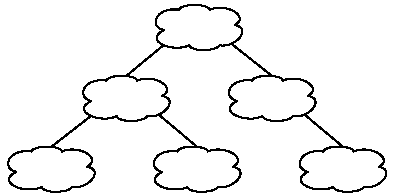
\includegraphics[width=2.2cm]{../img/tree.pdf} \\
\Emph{Graf}  & 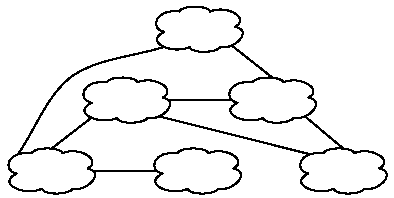
\includegraphics[width=2.2cm]{../img/graph.pdf} \\
\end{tabular}
\end{itemize}
{
\SlideFontTiny \vspace{1em }\hskip2em
Mer om listor \& träd \href{http://cs.lth.se/edaa01vt}{fördjupningskursen}. 
Mer om träd, grafer i \href{http://cs.lth.se/edaa40}{Diskreta strukturer.}
}

\end{Slide} 


\begin{Slide}{Vad är en vektor?}\SlideFontSmall
En \Emph{vektor}\footnote{Vektor kallas ibland på svenska även \href{https://sv.wikipedia.org/wiki/F\%C3\%A4lt_\%28datastruktur\%29}{fält}, men det skapar stor förvirring eftersom det engelska ordet \emph{field} ofta används för \emph{attribut} (förklaras senare).} 
\Eng{vector, \href{https://en.wikipedia.org/wiki/Array_data_structure}{array}} är en \Emph{samling} som är \Alert{snabb} att \Emph{indexera} i. 
Åtkomst av element sker med \code{apply(platsnummer)}: 

\begin{REPL}
scala> val heltal = Vector(42, 13, -1, 0 , 1)
heltal: scala.collection.immutable.Vector[Int] = Vector(42, 13, -1, 0, 1)

scala> heltal.apply(0)
res0: Int = 42

scala> heltal(1)    // man kan skippa .apply
res1: Int = 13

scala> heltal(5)
java.lang.IndexOutOfBoundsException: 5
  at scala.collection.immutable.Vector.checkRangeConvert(Vector.scala:132)
\end{REPL}
Utelämnar du \code{.apply} så gör kompilatorn anrop av \code{apply} ändå om det går.
\end{Slide}

\begin{Slide}{En konceptuell bild av en vektor}

\begin{REPLnonum}
scala> val heltal = Vector(42, 13, -1, 0 , 1)
\end{REPLnonum}

\begin{tikzpicture}[font=\ttfamily]
\matrix [matrix of nodes, row sep=0, column 2/.style={nodes={rectangle,draw,minimum width=3em}}] (var) at (0cm, 2.8cm)
{
heltal   &  \makebox(16,12){ }\\
};
\matrix [matrix of nodes, draw=black,row sep=0, column 2/.style={nodes={rectangle,draw,minimum width=4em}}] (vec) at (4cm, 1cm)
{
\textit{plats} &  \\
0   &  \makebox(16,12){42}\\
1   &  \makebox(16,12){13}\\
2   &  \makebox(16,12){-1}\\
3   &  \makebox(16,12){0}\\
4   &  \makebox(16,12){1}\\
};
\filldraw[black] (0.7cm,2.8cm) circle (3pt) node[] (ref) {};
 \draw [arrow] (ref) -- (vec);
\end{tikzpicture}

\vspace{1em} Elementen ligger på rad någonstans i minnet.
\end{Slide}



\begin{Slide}{En samling strängar}

\begin{itemize}
\item En vektor kan lagra många värden av samma typ. 
\item Elementen kan vara till exempel heltal eller strängar. 
\item Eller faktiskt vad som helst. 
\end{itemize}

\begin{REPL}
scala> val grönsaker = Vector("gurka","tomat","paprika","selleri")
grönsaker: scala.collection.immutable.Vector[String] = Vector(gurka, tomat, paprika, selleri)

scala> val g = grönsaker(1)
g: String = tomat

scala> val xs = Vector(42, "gurka", true, 42.0)
xs: scala.collection.immutable.Vector[Any] = Vector(42, gurka, true, 42.0)


\end{REPL}

\end{Slide}


\begin{Slide}{Loopa genom elementen i en vektor}
En \code{for}-\Emph{sats} som skriver ut alla element i en vektor:
\begin{REPL}
scala> val grönsaker = Vector("gurka","tomat","paprika","selleri")

scala> for (g <- grönsaker) println(g)
gurka
tomat
paprika
selleri

\end{REPL}

\end{Slide}


\begin{Slide}{Bygga en ny samling från en befintlig med for-uttryck}
Ett \code{for}-\code{yield}-\Emph{uttryck} som \Emph{skapar en \Alert{ny} samling}.

\begin{Code}[basicstyle=\ttfamily\fontsize{12}{14}\selectfont]
for (g <- grönsaker) yield "god " + g
\end{Code}

\begin{REPL}
scala> val grönsaker = Vector("gurka","tomat","paprika","selleri")

scala> for (g <- grönsaker) yield "god " + g
res0: scala.collection.immutable.Vector[String] = 
  Vector(god gurka, god tomat, god paprika, god selleri)

scala> val åsikter = for (g <- grönsaker) yield s"god $g"
åsikter: scala.collection.immutable.Vector[String] = 
  Vector(god gurka, god tomat, god paprika, god selleri)
\end{REPL}

\end{Slide}


\begin{Slide}{Samlingen \code{Range} håller reda på intervall}
\begin{itemize}
\item Med en \code{Range(start, slut)} kan du skapa ett intervall: \\ från och med \code{start} till (men inte med) \code{slut}
\end{itemize}

\begin{REPLnonum}
scala> Range(0, 42)
res0: scala.collection.immutable.Range = 
  Range(0, 1, 2, 3, 4, 5, 6, 7, 8, 9, 10, 11, 12, 13, 14, 
    15, 16, 17, 18, 19, 20, 21, 22, 23, 24, 25, 26, 27, 28, 
    29, 30, 31, 32, 33, 34, 35, 36, 37, 38, 39, 40, 41)
\end{REPLnonum}

\begin{itemize}
\item Men alla värden däremellan skapas inte förrän de behövs:
\end{itemize}

\begin{REPL}
scala> val jättestortIntervall = Range(0, Int.MaxValue)
jättestortIntervall: scala.collection.immutable.Range = Range(0, 1, 2, 3, 4, 5, ...

scala> jättestortIntervall.end
res1: Int = 2147483647

scala> jättestortIntervall.toVector
java.lang.OutOfMemoryError: GC overhead limit exceeded
\end{REPL}

\end{Slide}

\begin{Slide}{Loopa med Range}
\code{Range} används i for-lopar för att hålla reda på antalet rundor.
\begin{REPLnonum}
scala> for (i <- Range(0, 6)) print(" gurka " + i)
 gurka 0 gurka 1 gurka 2 gurka 3 gurka 4 gurka 5 
\end{REPLnonum}
Du kan skapa en \code{Range} med \code{until} efter ett heltal:
\begin{REPLnonum}
scala> 1 until 7
res1: scala.collection.immutable.Range = 
  Range(1, 2, 3, 4, 5, 6)

scala> for (i <- 1 until 7) print(" tomat " + i) 
 tomat 1 tomat 2 tomat 3 tomat 4 tomat 5 tomat 6

\end{REPLnonum}
\end{Slide}

\begin{Slide}{Loopa med Range skapad med \texttt{to}}

Med \code{to} efter ett heltal får du en \code{Range} till och \Emph{med} sista:
\begin{REPLnonum}
scala> 1 to 6
res2: scala.collection.immutable.Range.Inclusive = 
  Range(1, 2, 3, 4, 5, 6)

scala> for (i <- 1 to 6) print(" gurka " + i) 
 gurka 1 gurka 2 gurka 3 gurka 4 gurka 5 gurka 6
 
\end{REPLnonum}


\end{Slide}



\begin{Slide}{Vad är en \code{Array} i JVM?}


\begin{itemize}
\item En \code{Array} liknar en \code{Vector} men har en särställning i JVM:
\begin{itemize}
\item Lagras som en sekvens i minnet på efterföljande adresser.
\item \Emph{Fördel}: snabbaste samlingen för element-access i JVM.
\item Men det finns en hel del \Alert{nackdelar} som vi ska se senare.
\end{itemize}

\end{itemize}

\begin{REPLnonum}
scala> val heltal = Array(42, 13, -1, 0 , 1)
\end{REPLnonum}

\begin{tikzpicture}[font=\ttfamily,scale=0.75, every node/.style={scale=0.75}]
\matrix [matrix of nodes, row sep=0, column 2/.style={nodes={rectangle,draw,minimum width=3em}}] (var) at (0cm, 2.8cm)
{
heltal   &  \makebox(16,12){ }\\
};
\matrix [matrix of nodes, draw=black,row sep=0, column 2/.style={nodes={rectangle,draw,minimum width=4em}}] (vec) at (4cm, 1cm)
{
\textit{plats} &  \\
0   &  \makebox(16,12){42}\\
1   &  \makebox(16,12){13}\\
2   &  \makebox(16,12){-1}\\
3   &  \makebox(16,12){0}\\
4   &  \makebox(16,12){1}\\
};
\filldraw[black] (0.7cm,2.8cm) circle (3pt) node[] (ref) {};
 \draw [arrow] (ref) -- (vec);
\end{tikzpicture}
\end{Slide}



\Subsection{Huvudprogram med \texttt{main} i Scala och Java}

\begin{Slide}{Ett minimalt program i Scala och Java}

\begin{REPLnonum}
scala> println("Hello World!")
Hello World!
\end{REPLnonum}

\begin{Code}
// this is Scala 

object Hello {
  def main(args: Array[String]): Unit = {
    println("Hejsan scala-appen!")
  }
}
\end{Code}


\begin{Code}[language=Java]
// this is Java 

public class Hi {
    public static void main(String[] args) {
        System.out.println("Hejsan Java-appen!");
    }
}
\end{Code}

\end{Slide}


\begin{Slide}{Loopa genom en samling med en \texttt{while}-sats}
\end{Slide}


\begin{Slide}{Loopa genom argumenten i ett Scala-huvudprogram}
\end{Slide}


\begin{Slide}{Loopa genom argumenten i ett Java-huvudprogram}
\end{Slide}



\Subsection{Algoritmer}

\begin{Slide}{Vad är en algoritm?}
En \href{https://sv.wikipedia.org/wiki/Algoritm}{algoritm} är en sekvens av instruktioner\\ som beskriver hur man löser ett problem \\
\vspace{2em}
Exempel: \\ ~matrecept \\ \pause ~uppdatera highscore i ett spel \\ ~...
\begin{tikzpicture}[overlay]
\node[xshift=0.8\textwidth, scale=1.6] at (0,0) {XX};%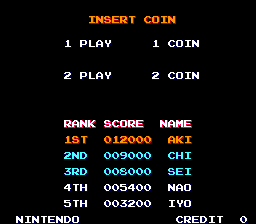
\includegraphics[width=0.25\textwidth]{img/highscore}};
\end{tikzpicture}
\end{Slide}

\begin{Slide}{Algoritmexempel: PRODUKTEN AV $n$ TAL}
\end{Slide}


\Subsection{Funktioner och procedurer skapar struktur}

\begin{Slide}{Block}\SlideFontSmall
Kapslar in många satser.

Vad är ett block?
I Scala (till skillnad från många andra språk) har ett block har ett värde 

\end{Slide}

\begin{Slide}{Block kan ha lokala variabler}\SlideFontSmall
Synlighetsregler etc
\end{Slide}


\begin{Slide}{Funktioner}\SlideFontSmall
\end{Slide}

\begin{Slide}{Parameter och argument}\SlideFontSmall
\end{Slide}

\begin{Slide}{Procedurer}\SlideFontSmall
\begin{itemize}
\item En \Emph{procedur} är en funktion som \Alert{gör} något intressant, men som \Alert{inte} lämnar något intressant returvärde.
\item Exempel på befintlig procedur: \code{println("hej")}
\item Du \Emph{deklarerar egna procedurer} genom att ange \texttt{\Alert{Unit}} som returvärdestyp. Då ges värdet \texttt{\Alert{()}} som betyder ''inget''.
\end{itemize}
\begin{REPL}
scala> def hej(x: String): Unit = println(s"Hej på dej $x!")
hej: (x: String)Unit

scala> hej("Herr Gurka")
Hej på dej Herr Gurka!

scala> val x = hej("Fru Tomat")
Hej på dej Fru Tomat!
x: Unit = ()
\end{REPL}
\begin{itemize}
\item Det som \Alert{görs} kallas (sido)\Emph{effekt}. Ovan är utskriften själva effekten.
\item Funktioner kan också ha sidoeffekter. De kallas då \Alert{oäkta} funktioner.
\end{itemize}
\end{Slide}

\begin{Slide}{Ingenting är faktiskt någonting i Scala}
I många språk (Java, C, C) är funktioner som saknar värden speciella. I Java finns nyckelordet  \jcode{void} men inte i Scala. I Scala är procedurer inte speciell efter som de faktisk returnerar ett värde som representerar ingenting, nämligen () som är av typen Unit. På så sätt blir procedurer inget undantag utan följer vanliga regler för syntax och semantik som för alla andra funktioner.

\url{https://en.wikipedia.org/wiki/Void_type}

\url{https://en.wikipedia.org/wiki/Unit_type}
\end{Slide}

\begin{Slide}{Abstraktion: Problemlösning genom nedbrytning i enkla funktioner och procedurer som kombineras}\SlideFontSmall
\begin{itemize}
\item En av de allra viktigaste principerna inom programmering är \Emph{funktionell nedbrytning} där  \Emph{underprogram} i form av funktioner och procedurer skapas för att bli byggstenar som kombineras till mer avancerade funktioner och procedurer.

\item Genom de namn som definieras skapas \Emph{återanvändbara abstraktioner} som kapslar in det funktionen gör. 

\item Problemet blir med bra byggblock lättare att lösa.

\item Abstraktioner som beräknar eller gör \Emph{en enda, väldefinierad sak} är enklare att använda, jämfört med de som gör många, helt olika saker.

\item Abstraktioner med \Emph{välgenomtänkta namn} är enklare att använda, jämfört med kryptiska eller missvisande namn.
\end{itemize}

\end{Slide}

\begin{Slide}{Exempel på funktionell nedbrytning}
$<<$kvadrat, stapel, rutnät i kojo$>>$ 
\end{Slide}


\begin{Slide}{Paket}
$<<$paket skapar katalogstruktur för kodfiler$>>$ 
\end{Slide}

\begin{Slide}{Jar-filer}
$<<$liknar zip-filer; packar ihop bytekod i en enda fil för enkel distribution$>>$ 
\end{Slide}

\subsection{Att göra denna vecka}


%%%
\frame{\frametitle{Att göra i Vecka \vecka: Förstå grundläggande kodstrukturer}
\begin{enumerate}
\item Laborationer är \Alert{obligatoriska}.\\ Ev. sjukdom måste anmälas \Alert{före} till kursansvarig!
\item Gör övning \texttt{programs}
\item OBS! Ingen lab denna vecka w02. Använd tiden att komma ikapp om du ligger efter!
\item Träffas i samarbetsgrupper och hjälp varandra att förstå.
\item Om ni inte redan gjort det: Gör klart \href{https://github.com/bjornregnell/lth-eda016-2015/tree/master/assignments}{samarbetskontrakt} och visa för handledare på resurstid.
\item \Alert{Koda på resurstiderna} och få hjälp och tips! 
\end{enumerate}
}










\Lecture{3}{Funktioner, Objekt}
%!TEX encoding = UTF-8 Unicode
%!TEX root = ../lect-week03.tex


\Subsection{Funktioner}



\begin{Slide}{Deklarera funktioner}
\begin{itemize}
\item En parameter, och sedan två parametrar:
\begin{REPL}
scala> :paste
  def öka(a: Int): Int = a + 1
  def öka(a: Int, b: Int) = a + b
  
scala> öka(1)
res0: Int = 2

scala> öka(1,1)
res1: Int = 2

\end{REPL}
\item Båda funktionerna ovan kan finnas samtidigt! Trots att de har samma namn är de \Alert{olika} funktioner; kompilatorn kan skilja dem åt med hjälp av de olika parameterlistorna.

\item Detta kallas \Emph{överlagring} \Eng{overloading} av funktioner.

\end{itemize}
\end{Slide} 


\begin{Slide}{Tom parameterlista och inga parametrar}\SlideFontSmall
\begin{itemize}
\item Om en funktion deklareras med tom parameterlista \code{()} kan den anropas på två sätt: med och utan tomma parenteser.
\begin{REPL}
scala> def tomParameterLista() = 42

scala> tomParameterLista()
res2: Int = 42

scala> tomParameterLista
res3: Int = 42
\end{REPL}

\item Men om parameterlista saknas får man \Alert{inte} använda \code{()} vid anrop:

\begin{REPL}

scala> def ingenParameterLista = 42

scala> ingenParameterLista
res4: Int = 42

scala> ingenParameterLista()
<console>:13: error: Int does not take parameters
       ingenParameterLista()
\end{REPL}

\end{itemize}
\end{Slide} 


\begin{Slide}{Funktioner med default-argument}\SlideFontSmall

\begin{itemize}
\item Vi kan ofta åstadkomma något som liknar överlagring, men med en enda funktion, om vi i stället använder \Emph{default-argument}:
\begin{REPLnonum}
scala> def inc(a: Int, b: Int = 1) = a + b
inc: (a: Int, b: Int)Int

scala> inc(42, 2)
res0: Int = 44

scala> inc(42, 1)
res1: Int = 43

scala> inc(42)
res2: Int = 43

\end{REPLnonum}
\item Om argumentet utelämnas och det finns ett default-argumentet, så är det default-argumentet som appliceras på parametern.
\end{itemize}
\end{Slide} 


\begin{Slide}{Stackminne och Heapminne}\SlideFontSmall
Minnet är uppdelat i två delar:
\begin{itemize}
\item \Emph{Stackminne}: På stacken läggs en \Emph{aktiveringspost} \Eng{stack frame\footnote{\href{https://en.wikipedia.org/wiki/Call_stack}{en.wikipedia.org/wiki/Call\_stack}}, activation record} för varje funktionsanrop med plats för parametrar och lokala variabler. Aktiveringsposten raderas när returvärdet har levererats. Stacken växer vid nästlade funktionsanrop, då en funktion i sin tur anropar en annan funktion. 

\item \Emph{Heapminne}: I heapminnet\footnote{\href{https://en.wikipedia.org/wiki/Memory_management}{en.wikipedia.org/wiki/Memory\_management}}$^{,}$\footnote{Ej att förväxlas med datastrukturen heap  \href{https://sv.wikipedia.org/wiki/Heap}{sv.wikipedia.org/wiki/Heap}} sparas alla objekt (data) som allokeras under körning. Heapminnet städas vid tillfälle av skräpsamlaren \Eng{garbage collector}, och minne som inte används längre frigörs. \\\vspace{0.5em}
\href{http://stackoverflow.com/questions/1565388/increase-heap-size-in-java}{stackoverflow.com/questions/1565388/increase-heap-size-in-java}
\end{itemize}
\end{Slide} 


\begin{Slide}{Aktiveringspost}\SlideFontSmall
Nästlade anrop ger växande stackminne.
\begin{REPL}
scala> :paste
def f(): Unit = { val n = 5; g(n, 2 * n) }
def g(a: Int, b: Int): Unit = { val x = 1; h(x + 1, a + b) }
def h(x: Int, y: Int): Unit = { val z = x + y; println(z) }

scala> f()

\end{REPL}

\Alert{Stacken}

\begin{tabular}{|r | l | l |} \hline

variabel & värde & Vilken aktiveringspost? \\ \hline \hline
\pause
 n & 5 & f \\ \hline
 \pause 
 a & 5 & g \\
 b & 10 &  \\
 x & 1  &  \\  \hline
 \pause 
 x & 2  & h \\
 y & 15 &  \\
 z & 17 & \\ 
\end{tabular}
\end{Slide} 


\begin{Slide}{Lokala funktioner}
\end{Slide} 



\begin{Slide}{Värdeanrop och namnanrop}
\begin{itemize}
\item 
\end{itemize}
\end{Slide} 



\begin{Slide}{Uppdelad parameterlista}
\begin{itemize}
\item 
\end{itemize}
\end{Slide} 


\begin{Slide}{Skapa din egen kontrollstruktur}
\begin{itemize}
\item 
\end{itemize}
\end{Slide} 


\begin{Slide}{Funktioner med namngivna argument}
\begin{itemize}
\item 
\end{itemize}
\end{Slide} 



\begin{Slide}{Funktioner är äkta värden i Scala}
\begin{itemize}
\item En funktioner är ett äkta värde; vi kan till exempel tilldela en variabel ett funktionsvärde:
\item Funktioner har en typ precis som alla värden:
\end{itemize}
\end{Slide} 



\begin{Slide}{Anonyma funktioner}
\begin{itemize}
\item 
\end{itemize}
\end{Slide}




\begin{Slide}{Applicera funktioner på element i samlingar}
\begin{itemize}
\item 
\end{itemize}
\end{Slide} 




\begin{Slide}{Stegade funktioner, ''Curry-funktioner''}
\begin{itemize}
\item 
\end{itemize}
\end{Slide} 





\Subsection{Objekt}

\begin{Slide}{Objekt som modul}
\begin{itemize}
\item Ett \code{object} användas ofta för att samla \Emph{medlemmar} som hör ihop och ge dem en egen \Emph{namnrymd}. 
\item Medlemmarna kan vara t.ex.: 
\begin{itemize}
\item  \code{val} \item \code{var} \item \code{def} 
\end{itemize}
\item Ett sådant objekt kallas även för \Emph{modul}.\footnote{
Även paket som skapas med \code{package} har en egen namnrymd och är därmed också en slags modul. Objekt kan alltså i Scala användas som ett alternativ till paket; en skillnad är att objekt kan ha tillstånd och att objekt inte skapar underkataloger vid kompilering.  \href{https://en.wikipedia.org/wiki/Modular_programming}{en.wikipedia.org/wiki/Modular\_programming}}

\end{itemize}

\end{Slide}


\begin{Slide}{Vad är ett tillstånd?} 
\end{Slide} 

\begin{Slide}{Lata variabler och fördröjd evaluering} 
\end{Slide} 

\begin{Slide}{Vad är egentligen skillnaden mellan \texttt{val}, \texttt{lazy val}, \texttt{var}, \texttt{def}?} 

En funktion som finns inuti ett objekt är en \Emph{metod}.
\end{Slide} 


\Subsection{Funktioner är objekt}

\begin{Slide}{Programmeringsparadigm}
\end{Slide} 


\begin{Slide}{Funktioner är äkta objekt i Scala}
Scala visar hur man kan \Alert{förena} \Eng{unify} objekt-orientering och funktionsprogrammering på ett elegant \& pragmatiskt sätt: \\\vspace{2em}

\Emph{\Large En funktion är ett objekt \\ som har en \code{apply}-metod.}

\end{Slide} 



\Subsection{Rekursion}
\begin{Slide}{Rekursiva funktioner}
\end{Slide} 

\begin{Slide}{Rekursiva datastrukturer}
\end{Slide} 



\end{document}
